% ------------------------------------------------------------
% File: figures/fig-iteration-1-mask-popout.tex
% Iteration 1 mask callout: device mask -> gate mask -> dimensions
% ------------------------------------------------------------

\begin{figure}[htbp]
  \centering
  \begin{tikzpicture}[
    font=\footnotesize,
    callout/.style={dashed, line width=0.8pt},
    connector/.style={dashed, line width=0.45pt, opacity=0.45},
    imagebox/.style={draw, line width=0.4pt, inner sep=2pt},
    figlabel/.style={draw, fill=white, line width=0.35pt, inner xsep=4pt,
      inner ysep=2pt, font=\small\bfseries}
  ]
    % Manual adjustment controls:
    % - Device image size: change the width in the device \includegraphics.
    % - Red source box on device mask: change \devBoxLeft, \devBoxRight,
    %   \devBoxTop, and \devBoxBottom. These are fractions of the image width
    %   and height from the image edges.
    % - Red source box on the device mask: these are image fractions from
    %   the top-left of the device image. The current box is landscape and
    %   matches the physical aspect ratio of gate_mask.png.
    \def\devBoxLeft{0.305}
    \def\devBoxRight{0.685}
    \def\devBoxTop{0.250}
    \def\devBoxBottom{0.500}
    % - Blue source box on the gate mask: currently placed just right of
    %   centre height, over one recess region. Adjust these fractions after
    %   checking the compiled image.
    \def\gateBlueLeft{0.705}
    \def\gateBlueRight{0.845}
    \def\gateBlueTop{0.44}
    \def\gateBlueBottom{0.58}

    % Top-level device mask.
    \node[imagebox, anchor=north west] (device) at (0,0) {
      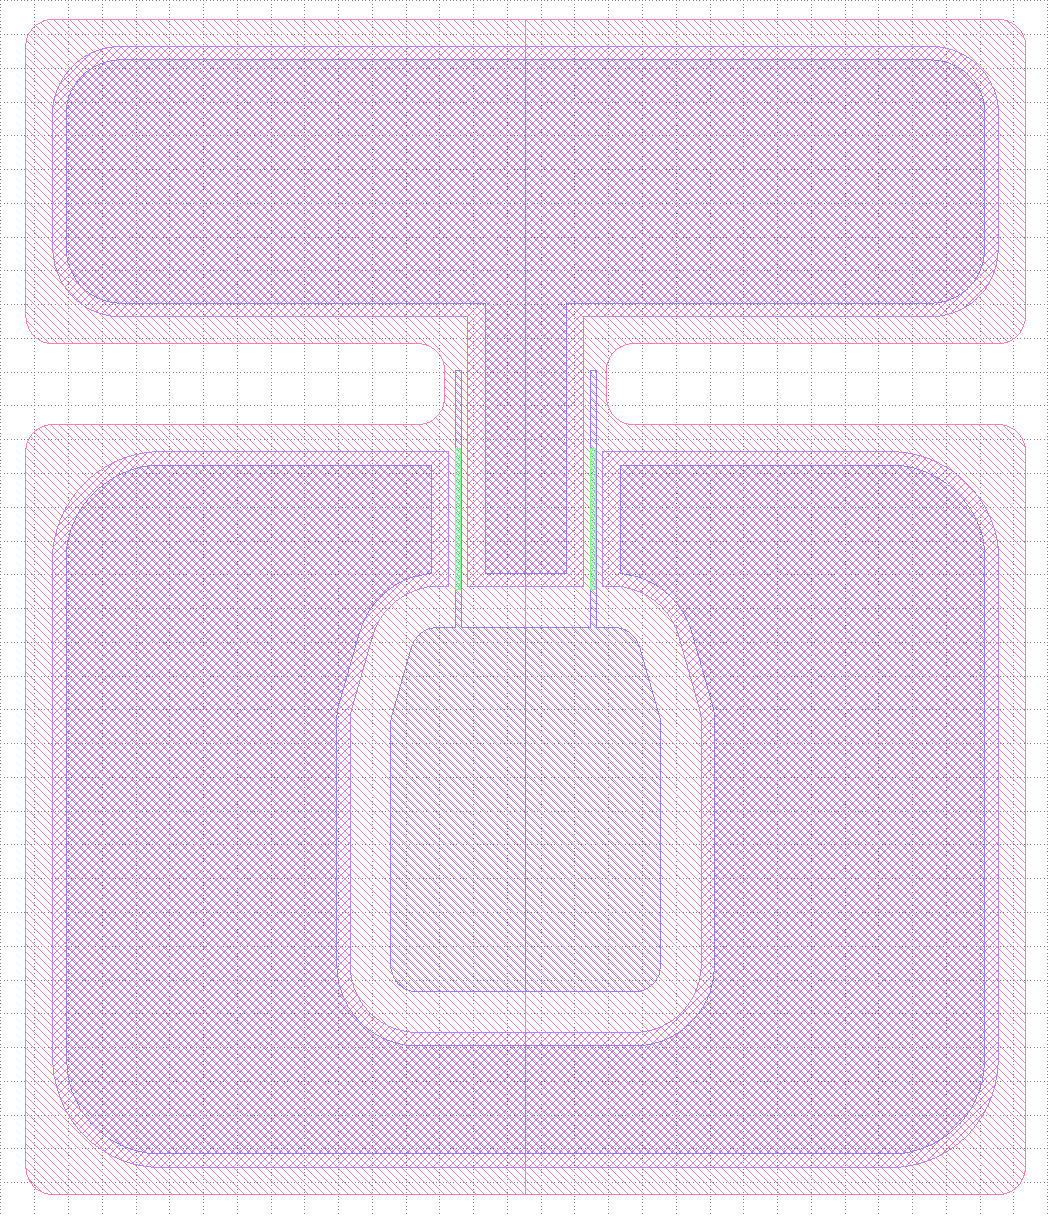
\includegraphics[width=0.28\linewidth]{figures/gate_recession/device_mask.png}
    };
    \node[figlabel, anchor=north, yshift=-1.5mm] (deviceLabel) at (device.south) {Single Device Mask};

    % Pop-out gate mask.
    \node[imagebox, anchor=north west] (gate) at (7.1,0) {
      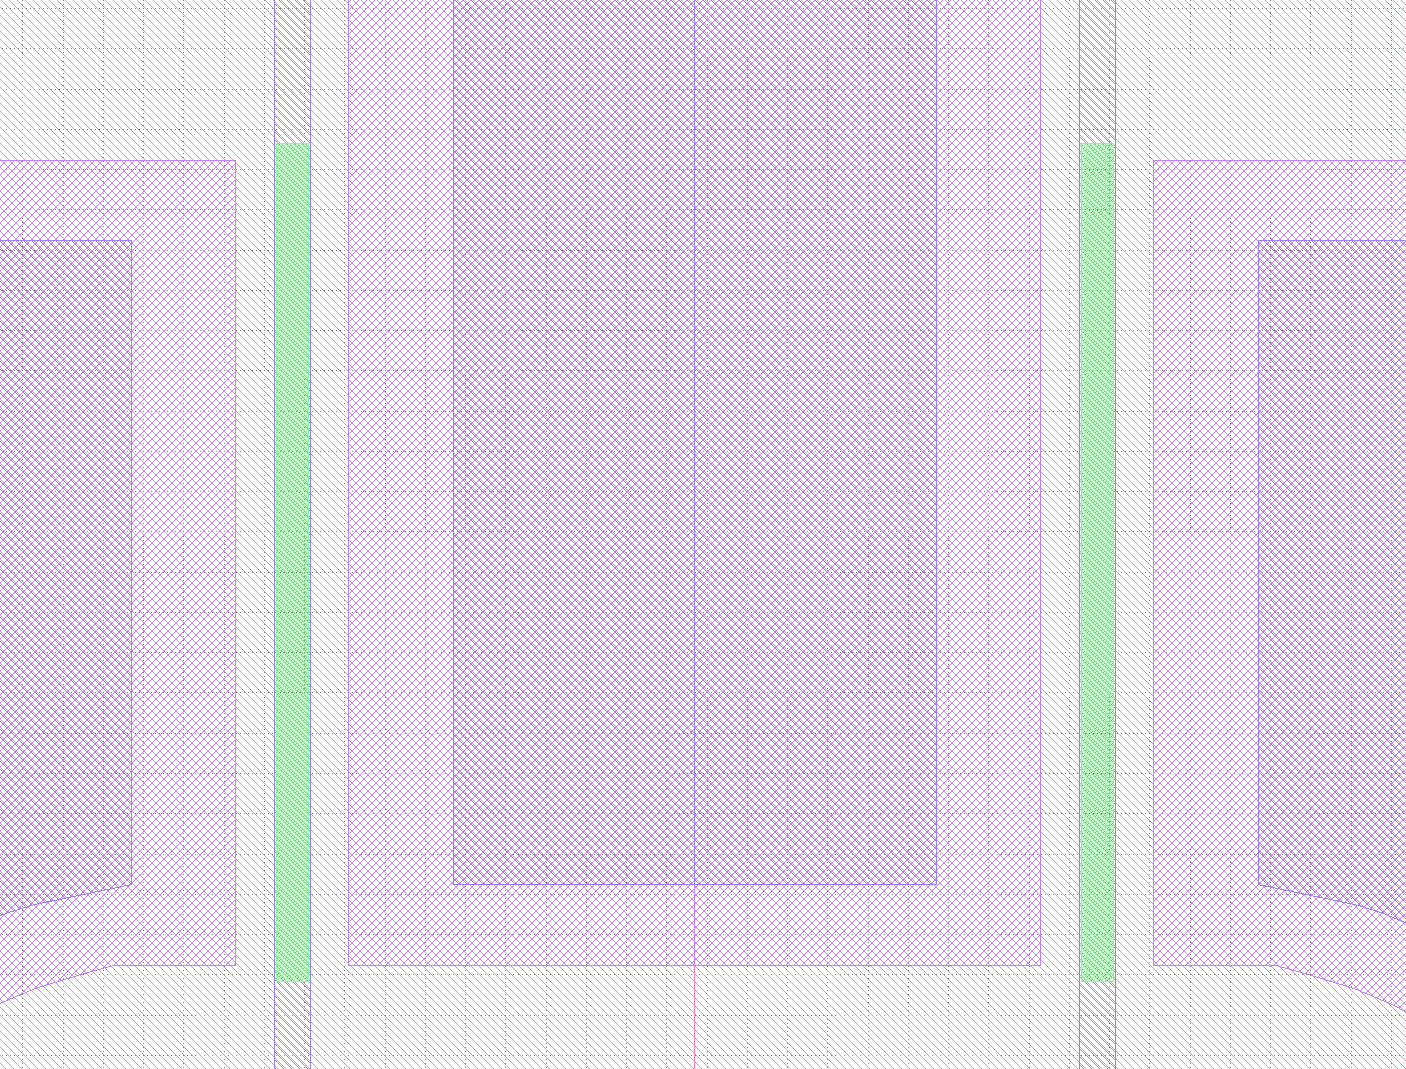
\includegraphics[width=0.426\linewidth]{figures/gate_recession/gate_mask.png}
    };
    \node[figlabel, anchor=north, yshift=-1.5mm] (gateLabel) at (gate.south) {Gate/Recess Mask Zoomed};

    % Lower dimensions pop-out.
    \node[imagebox, anchor=north] (dimensions) at ($(device.south west)!0.5!(gate.south east)+(0,-1.10)$) {
      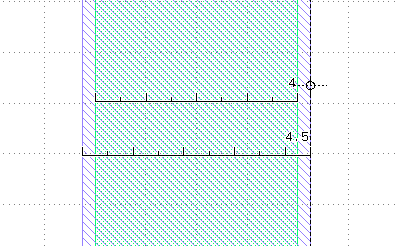
\includegraphics[width=0.64\linewidth]{figures/gate_recession/mask_dimensions.png}
    };
    \node[figlabel, anchor=north, yshift=-1.5mm] (dimensionsLabel) at (dimensions.south) {Gate/Recess Mask Dimensions};

    % Red source callout on the device mask.
    \path let \p1=(device.north west), \p2=(device.south east) in
      coordinate (deviceBoxNW) at ({\x1+\devBoxLeft*(\x2-\x1)}, {\y1+\devBoxTop*(\y2-\y1)})
      coordinate (deviceBoxNE) at ({\x1+\devBoxRight*(\x2-\x1)}, {\y1+\devBoxTop*(\y2-\y1)})
      coordinate (deviceBoxSW) at ({\x1+\devBoxLeft*(\x2-\x1)}, {\y1+\devBoxBottom*(\y2-\y1)})
      coordinate (deviceBoxSE) at ({\x1+\devBoxRight*(\x2-\x1)}, {\y1+\devBoxBottom*(\y2-\y1)});

    \draw[callout, red!75!black]
      (deviceBoxNW) rectangle (deviceBoxSE);

    % Pop-out target box on the gate mask. Currently surrounds the full image.
    \coordinate (gateRedNW) at ($(gate.north west)+(0.08,-0.08)$);
    \coordinate (gateRedNE) at ($(gate.north east)+(-0.08,-0.08)$);
    \coordinate (gateRedSW) at ($(gate.south west)+(0.08,0.08)$);
    \coordinate (gateRedSE) at ($(gate.south east)+(-0.08,0.08)$);
    \draw[callout, red!75!black]
      (gateRedNW) rectangle (gateRedSE);

    % Blue source callout on the gate mask.
    \path let \p1=(gate.north west), \p2=(gate.south east) in
      coordinate (gateBlueNW) at ({\x1+\gateBlueLeft*(\x2-\x1)}, {\y1+\gateBlueTop*(\y2-\y1)})
      coordinate (gateBlueNE) at ({\x1+\gateBlueRight*(\x2-\x1)}, {\y1+\gateBlueTop*(\y2-\y1)})
      coordinate (gateBlueSW) at ({\x1+\gateBlueLeft*(\x2-\x1)}, {\y1+\gateBlueBottom*(\y2-\y1)})
      coordinate (gateBlueSE) at ({\x1+\gateBlueRight*(\x2-\x1)}, {\y1+\gateBlueBottom*(\y2-\y1)});

    \draw[callout, blue!70!black]
      (gateBlueNW) rectangle (gateBlueSE);

    \coordinate (dimBlueNW) at ($(dimensions.north west)+(0.08,-0.08)$);
    \coordinate (dimBlueNE) at ($(dimensions.north east)+(-0.08,-0.08)$);
    \coordinate (dimBlueSW) at ($(dimensions.south west)+(0.08,0.08)$);
    \coordinate (dimBlueSE) at ($(dimensions.south east)+(-0.08,0.08)$);
    \draw[callout, blue!70!black]
      (dimBlueNW) rectangle (dimBlueSE);

    % Device mask -> gate mask pop-out connectors. These are drawn above the
    % device mask, then the gate/recess mask panel is redrawn over them.
    \draw[connector, red!75!black]
      (deviceBoxNW) --
      (gateRedNW);
    \draw[connector, red!75!black]
      (deviceBoxNE) --
      (gateRedNE);
    \draw[connector, red!75!black]
      (deviceBoxSW) --
      (gateRedSW);
    \draw[connector, red!75!black]
      (deviceBoxSE) --
      (gateRedSE);

    % Redraw the gate/recess mask panel so red connector lines sit beneath it.
    \node[imagebox, anchor=north west] at (gate.north west) {
      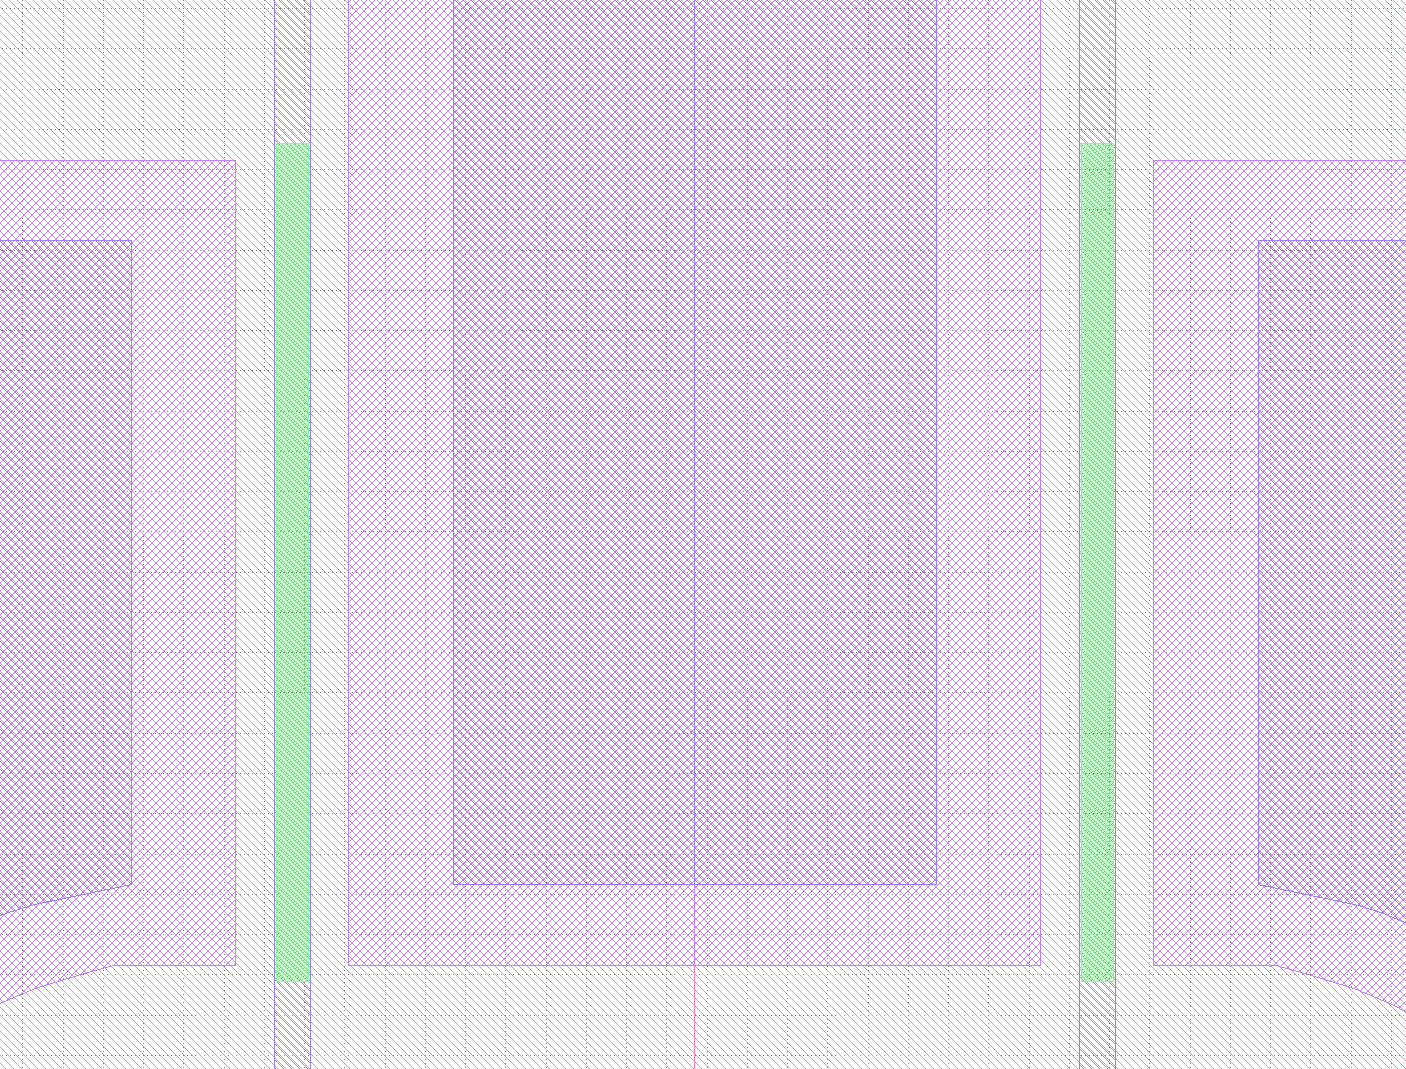
\includegraphics[width=0.426\linewidth]{figures/gate_recession/gate_mask.png}
    };
    \draw[callout, red!75!black]
      (gateRedNW) rectangle (gateRedSE);
    \draw[callout, blue!70!black]
      (gateBlueNW) rectangle (gateBlueSE);

    % Gate mask -> dimensions pop-out connectors. These are drawn above the
    % gate/recess mask, then the dimensions panel is redrawn over them.
    \draw[connector, blue!70!black]
      (gateBlueNW) --
      (dimBlueNW);
    \draw[connector, blue!70!black]
      (gateBlueNE) --
      (dimBlueNE);
    \draw[connector, blue!70!black]
      (gateBlueSW) --
      (dimBlueSW);
    \draw[connector, blue!70!black]
      (gateBlueSE) --
      (dimBlueSE);

    % Redraw the dimensions panel so blue connector lines sit beneath it.
    \node[imagebox, anchor=north] at (dimensions.north) {
      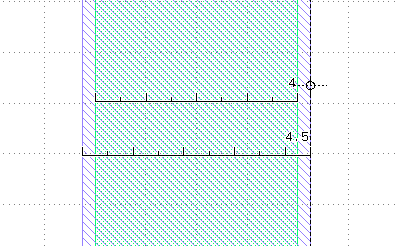
\includegraphics[width=0.64\linewidth]{figures/gate_recession/mask_dimensions.png}
    };
    \draw[callout, blue!70!black]
      (dimBlueNW) rectangle (dimBlueSE);

    % Redraw labels above connector lines.
    \node[figlabel, anchor=north, yshift=-1.5mm] at (device.south) {Single Device mask};
    \node[figlabel, anchor=north, yshift=-1.5mm] at (gate.south) {Gate/Recess Mask Zoomed};
    \node[figlabel, anchor=north, yshift=-1.5mm] at (dimensions.south) {Gate/Recess Mask Dimensions};
  \end{tikzpicture}

  \vspace{2mm}
  \caption{Iteration 1 mask structure with device-level, gate/recess, and
  dimensioned views.}
  \label{fig:iteration-1-mask}
\end{figure}
